\section{Program Logic}
\label{sec:logic}

%\indent
% We first design a program logic for \sparc{} program,
% which doesn't consider refinement verification.
% In this section, we use such program logic to present
% how our logic handles the features of \sparc{}.
In this section,
we use a simplified version of our program logic
that doesn't support refinement verification to
present how our logic handles the
features of \sparc{}.

% In this section,
% we introduce the assertion language
% and program logic designed for \sparc{} program.
% %We will elaborate how our logic handles the features of \sparc{} in detail.
% %Finally, we will present our semantic approach for establishing soundness.

\subsection{Assertions}
\label{subsec:assertions}

\begin{center}
	$
		\begin{array}{rrcl}
			\textit{(Asrt)} & \astP, \astQ & \define &
			\aemp \sepline
			\msto{l}{\val} \sepline
			\regst{\regN}{\val} \sepline
			\dlyregst{t}{\sr}{\word} \sepline
			\asrttm{p} \\
			& & \ \ \ | &
			\frmst{\cwp}{F} \sepline
			\astP \wedge \astQ \sepline
			\astP \vee \, \astQ \sepline
			\astP \sepstar \astQ \\
			& & \ \ \ | &
			\aexp \addrEq \val \sepline
			\oexp = \val \sepline
			\forall x. \, \astP \sepline
			\exists x. \, \astQ \sepline
            \dots
		\end{array}
	$
	\figurecaption{Syntax of Assertions}
	\label{fig:Syntax of Assertions}
	\vspace{-0.5em}
\end{center}

% \begin{figure*}[!t]
% 	\centering
% 	\small
% 	\vspace{-0.5em}
% 	\small
% 	$
% 		\begin{array}{rrcl}
%             \textit{(Asrt)} & \astP, q & \define &
%             \aemp \sepline
% 			\msto{l}{\val} \sepline
% 			\regst{\regN}{\val} \sepline
% 			\dlyregst{t}{\sr}{\word} \sepline

% 			\asrttm{p} \sepline
%             \frmst{\cwp}{F} \\ %\sepline \\
%             & &\ \,\sepline &
% 			%\apure{p} \sepline
% 			\astP \wedge \astQ \sepline
% 			\astP \vee \, \astQ \sepline
% 			\astP \sepstar \astQ \sepline
% 			\aexp \addrEq \val \sepline
% 			\oexp = \val \sepline
% 			\forall x. \, \astP \sepline
% 			\exists x. \, \astQ \sepline
%             \dots
% 		\end{array}
% 	$
% 	\caption{Syntax of Assertions}
% 	\label{fig:Syntax of Assertions}
% 	\vspace{-0.5em}
% \end{figure*}

\begin{figure*}[!t]
	\centering
	\vspace{-0.5em}
	$
		\begin{array}{l}
			\begin{array}{lcl}
				\asrtmodel{\state}{\aemp} & \define & S.M = \emptyset \, \wedge \, S.Q.R = \emptyset \\
				
				\asrtmodel{\state}{l \mapsto \val} & \define &
					S.M = \{l \rightsquigarrow \val\} \, \wedge \,
                S.Q.R = \emptyset \\
				
				\asrtmodel{\state}{\regst{\regN}{\val}} & \define &
				S.Q.R = \{\regN \rightsquigarrow \val\}
                \, \wedge \, \regN \notin \dom(\state.\DBuf)
                \, \wedge \, \state.\mem = \emptyset \\
				
				\asrtmodel{\state}{\dlyregst{t}{\sr}{\word}} & \define &
                    \exists k,\RFile',\DBuf'.\,
                    0 \le k \le t\!+\!1
                    \land
                    \DstepN{k}{(\RFile, \DBuf)}{(\RFile', \DBuf')}
                    \land
                    \\ & & \hspace*{16ex}
                    \left(
                      \asrtmodel{(\mem, (\RFile', F), \DBuf')}{\regst{\sr}{\word}}
                    \right)
                    \land \noDup\DBuf\sr
                  \\
                  & & \hspace*{16ex}
                  \text{where }\state = (\mem, (\RFile, \Wstack), \DBuf)
                  \\

				\asrtmodel{\state}{\nxtAst\astP} & \define &
				\exists \RFile', \DBuf'. \;
                \left(
                  \asrtmodel{(\mem, (\RFile', \Wstack), \DBuf')}\astP
                \right)
                \land
                %\exedelay(R', D') = (S.Q.R, S.D)
                \Dstep{(\RFile', \DBuf')}{(\RFile, \DBuf)}
                  \\
                  & & \hspace*{16ex}
                  \text{where }\state = (\mem, (\RFile, \Wstack), \DBuf)
                  \\
				
				\asrtmodel{\state}{\frmst{\cwp}{\Wstack}} & \define &
				\left(\state \models \regst{\regcwp}{\cwp}\right) \, \wedge
                \exists \Wstack'.\, \Wstack \lstApp\Wstack' = S.Q.F \\

                \asrtmodel{S}{\aexpeq{\aexp}{\val}} & \define &
                \evalR{\aexp}{S.Q.R} = \val \, \wedge \, \wordaligned{(\val)} \\

                \asrtmodel{S}{\oexpeq{\oexp}{\val}} & \define & \evalR{\oexp}{S.Q.R} = \val \\
				
				\asrtmodel{S}{p_1 * p_2} & \define &
				\exists S_1, S_2. \; S_1 \models p_1 \, \wedge \, S_2 \models p_2 \, \wedge \,

				S = S_1 \uplus S_2

			\end{array} \\
			
			\\
			{\color{blue}
			\mem_1\!\perp\!\mem_2 \ \define \
			(\dom(\mem_1)\cap\dom(\mem_2)) = \emptyset
			\qquad \ \
			\RFile_1\!\perp\!\RFile_2 \ \define \
			(\dom(\RFile_1)\cap\dom(\RFile_2)) = \emptyset
			}
			\\
			\\[-5pt]
			
			\state_1 \!\uplus\! \state_2 \ \define \
			\left\{
				\begin{array}{ll}
					(\mem_1 \!\cup\! \mem_2, (\RFile_1 \!\cup\! \RFile_2, \Wstack), \DBuf)
						 &  \quad \textbf{if} \;
						 		% {\color{blue}
								%  \dom(\mem_1) \cap \dom(\mem_2) = \emptyset \land
								%  \dom(\RFile_1) \cap \dom(\RFile_2) = \emptyset}
								%  \land  \\

						 		\mem_1 \!\perp\! \mem_2
                                  \wedge  \RFile_1 \!\perp\! \RFile_2  \wedge   \\
					& \quad \quad  \state_1 \!=\! (\mem_1, (\RFile_1, \Wstack), \DBuf)
                                  \wedge \state_2 \!=\! (\mem_2, (\RFile_2, \Wstack), \DBuf) \\
					
					\\[-8pt]
					
					\undef & \quad \text{otherwise}
				\end{array}
			\right.

			\\
			\\
%			\DtoS\DBuf \ \define \
%			\left\{
%			\begin{array}{ll}
%				\{(n, \sr, \word)\} \cup \DtoS{\DBuf'}
%                    & \quad \textbf{if} \;
%                         \DBuf = (n, \sr, \word) \dbCons \DBuf' \\
%				
%				\\[-8pt]
%				
%				\emptyset & \quad \textbf{if} \; \DBuf = \nil
%			\end{array}
%			\right.
%            \\
%			
%			\\[-5pt]

			\dom(\DBuf) \ \define \
			\left\{
			\begin{array}{ll}
				\{\sr\} \cup \dom(\DBuf') & \quad \textbf{if} \;
                         \DBuf = (\tick, \sr, \word) \dbCons \DBuf' \\
				
				\\[-8pt]
				
				\emptyset & \quad \textbf{if} \; \DBuf = \nil
			\end{array}
			\right.
            \\
			
			\\[-8pt]
%
			\noDup\DBuf\sr \ \define \
			\left\{
			\begin{array}{ll}
				\sr\not\in\dom(\DBuf')
                    & \quad \textbf{if} \;
                         \DBuf = (\tick, \sr, \word) \dbCons \DBuf' \\
				
				\\[-8pt]
				
				\sr\neq\sr' \land \noDup{\DBuf'}\sr
                    & \quad \textbf{if} \;
                         \DBuf = (\tick, \sr', \word) \dbCons \DBuf' \\
				
				\\[-8pt]
				\textbf{True} & \quad \textbf{if} \; \DBuf = \nil
			\end{array}
			\right.
            \\
			
			\\[-5pt]

%			\noDup\DBuf\sr \ \define \
%             \forall n_1, n_2, \word_1, \word_2.
%             (n_1, \sr, \word_1) \!\in\! \DtoS\DBuf \land
%             (n_2, \sr, \word_2) \!\in\! \DtoS\DBuf
%             \Rightarrow
%             \\ \hspace*{55ex}
%             n_1 \!=\! n_2 \land \word_1 \!=\! \word_2
%%            \qquad
%%			\textbf{noDup} (\sr, lr) \ \define \
%%			\sr \notin lr \backslash \{\sr\}
%            \\
%			
%			\\[-5pt]
			
%			\substFld{S}{R', D'} \define (M, (R', F), D'),
%            \ \ \ \ \text{where } S = (M, (R, F), D)
%            \\
%            \\[-5pt]

            %\begin{array}{ll}
%                \begin{array}{lcl}
%                    \evalR{\oexp}{R} & \define &
%                    \left\{
%                        \begin{array}{ll}
%                            R(r) &\quad \cif \ \oexp = r \\
%                            \\[-8pt]
%                            w &\quad \cif \ \oexp = \word, \\
%                            & \quad \quad -4096 \leq \word \leq 4095 \\
%                            \\[-8pt]
%                            \perp &\quad \otherwise
%                        \end{array}
%                    \right.
%                \end{array} & \quad
%                \begin{array}{lcl}
%                    \evalR{\aexp}{R} & \define &
%                    \left\{
%                        \begin{array}{ll}
%                            \evalR{\oexp}{R} &\quad \cif \ \aexp = \oexp \\
%                            \\[-8pt]
%
%                            v_1 \!+\! v_2 &\quad \cif \ \aexp = r \!+\! \oexp,\
%                              R(r) \!=\! v_1 \\
%                            & \quad \quad \tand \ \evalR{\oexp}{R} = v_2 \\
%
%                            \\[-8pt]
%                            \perp &\quad \otherwise
%                        \end{array}
%                    \right.
%                \end{array}
%            \end{array}
		\end{array}
	$
	\caption{Semantics of Assertions}
	\label{fig:Semantics of Assertions}
	\vspace{-0.5em}
\end{figure*}

%\indent
We define the syntax of assertions in Fig.~\ref{fig:Syntax of Assertions},
and their semantics in Fig.~\ref{fig:Semantics of Assertions}.
We extend separation logic assertions with specifications of
delay buffers and register windows. Registers are like
variables in separation logic, but are treated as resources.
The assertion $\aemp$ says
that the memory and the register file are both empty.
$\msto{\loc}{\val}$ specifies a singleton memory cell
with value $\val$ stored in the address $l$.
$\regst{\regN}{\val}$ says that
$\regN$ is the only register in the register file
and it contains the value $\val$. Also
$\regN$ is {\em not} in the delay buffer.
Separating conjunction $\astP \sepstar \astQ$ has the
standard semantics as in separation logic \cite{separationlogic}.
%there is only one cell in register file
%that maps the register name $\regN$ to value $\word$ and $\regN$ is not in delay list.


%Our assertion language is shown in Fig. \ref{fig:Syntax of Assertions}.
%And the semantics of some of them are presented
%in Fig. \ref{fig:Semantics of Assertions}.

%\indent
%Assertion emp says
%that the memory and register file are both empty.
%$\msto{l}{\word}$ specifies a singleton memory cell
%with value $\word$ stored in address $l$.
%$\regst{\regN}{\word}$ says that
%there is only one cell in register file
%that maps the register name $\regN$ to value $\word$ and $\regN$ is not in delay list.

%Delayed writes cause uncertainty of special registers $\sr$
%in $\RFile$.
The assertion $\dlyregst{\tick}{\sr}{\word}$ describes a delayed
write in the delay buffer $\DBuf$. It describes the
uncertainty of $\sr$'s value in $\RFile$, which is unknown
for now but will become $\word$ in up to $\tick\!+\!1$ cycles.
%It says the value of $\sr$ in the register file is unknown, but
%it will become $\word$ in up to $\tick\!+\!1$ cycles.
We use $\DstepN{k}{\notCare}{\notCare}$
to represent $k$-step execution of the delayed writes in $\DBuf$.
It also requires that there be
at most one delayed write for a specific special register $\sr$
in $\DBuf$ (\ie{} $\noDup{\sr}{\DBuf}$).
This prevents more than one delayed write to
the same register within 4 instruction cycles, which practically
have no restrictions on programming.
By the semantics we have
$$
\regst{\sr}{\word} \,\Longrightarrow \dlyregst{\tick}{\sr}{\word}
\qquad
\dlyregst{\tick}{\sr}{\word} \,\Longrightarrow\,
\dlyregst{\tick\!+\!k}{\sr}{\word}
$$

The assertion $\nxtAst\astP$ allows us to reduce the uncertainty
by executing one step of the delayed writes.
It specifies states reachable after executing
one step of delayed writes from those states satisfying $\astP$.
Therefore we know:
$$
\nxtAst{(\dlyregst{0}{\sr}{\word})} \Longrightarrow
\regst{\sr}{\word}
\quad \
\nxtAst{(\dlyregst{\tick\!+\!1}{\sr}{\word})} \Longrightarrow
\dlyregst{\tick}{\sr}{\word}
$$
Also it's easy to see that if $\astP$ syntactically
does not contain sub-terms in the form of $\dlyregst{\tick}{\sr}{\word}$,
then $(\nxtAst\astP) \,\Longleftrightarrow \,\astP$.

The following lemma shows $\nxtAst{(\notCare)}$ is distributive
over separating conjunction.
\begin{lemma} %\mbox{}
\label{lemma:dly-sep-split}
$
\nxtAst{(\astP * \astQ)} \,\Longleftrightarrow\, (\nxtAst\astP) * (\nxtAst\astQ)\,.
$
%\end{enumerate}
\end{lemma}
The lemma can be proved following Lemma~\ref{lemma:RFileSplitExDelay}.


We use $\frmst{\cwp}{\Wstack}$ to describe the pointer
$\regcwp$ of the current register window and the frame
list as a circular stack.
Note that $\Wstack$ is just a prefix of the frame list,
since usually we do not need to know contents of
the full list. Here we use $\Wstack \lstApp \Wstack'$ to
represent the concatenation of lists $\Wstack$ and $\Wstack'$.
Therefore we have
$
\frmst{\cwp}{\Wstack \lstApp \Wstack'} \,\Longrightarrow\,
\frmst{\cwp}{\Wstack}
$\,.


The assertions $\aexpeq{\aexp}{\val}$ and $\oexpeq{\oexp}{\val}$
describe the value of $\aexp$ and $\oexp$ respectively. They are
intuitionistic assertions. Since $\aexp$ is used as an address,
we also require it to be properly aligned on a 4-byte boundary.
We define $\wordaligned{}$ to represent this restriction below.
The result of the address expression $\aexp$ may be a word, if
it's a pointer in code heap, or a memory address, if it's a location
of memory.
\[
	\wordaligned{(\val)} \define
	\exists \, \word. \,
	(\val = \word \, \lor \, \val = (\notCare, \word))
	\, \land \, \word\modOP{4} = 0
	% \exists \, \word. \,
	% (\val = \word \, \lor \, (\exists \, \block. \, \val = (\block, \word)))
	% \, \land \, \word\modOP{4} = 0
\]

\subsection{Inference Rules}
\label{subsec:inference rules}
\newcommand{\tinybftext}[1]{\textbf{\scriptsize{#1}}}

%\begin{figure}[!t]
%	\centering
%	\subfigure[]
%	{
%		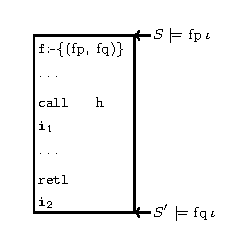
\includegraphics[width=35ex]{picture//funspec}
%		\label{fig:function specification}
%	}
%	\hspace{3em}
%	\subfigure[]
%	{
%		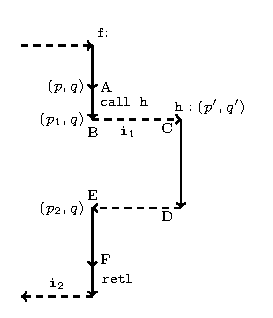
\includegraphics[width=38ex]{picture//CallReturnHandling}
%		\label{fig:call return handling}
%	}
%	\label{fig:Function Call/Return and Delayed-control-transfer Handling}
%	\caption{Function Call/Return and Delayed-control-transfer Handling}
%\end{figure}

%\indent
%We define a set of inference rules
%so that we can check \sparc{} code mechanized.
The code specification $\theta$ and code heap specification $\Psi$
are defined below:
\[
	\small
	\begin{array}{lccllccl}
		\text{(valList)} & \lgvl & \in & \text{list value}
			&
		\multicolumn{4}{l}
		{
			\quad
			\text{(pAsrt)} \ \
			\specpre,\specpost \in
			\text{valList} \rightarrow Asrt
		}
		% \specpre,\specpost &
		% 			\in & \text{valList} \rightarrow Asrt
		\\
		
		\text{(CdSpec)} & \Bspec & ::= & (\specpre, \specpost)
			& \quad
		
		\text{(CdHpSpec)} & \Cspec & ::= & \{\lab{} \rightsquigarrow \Bspec\}^{*}
	\end{array}
\]

The code heap specification $\Psi$ maps the code labels
for basic blocks to their specifications $\theta$,
which is a pair of pre- and post-conditions.
Instead of using normal assertions, the pre- and
post-conditions are assertions parameterized over
a list of values $\lgvl$. They play the role
of auxiliary variables --- Feeding the pre-
and the post-conditions with the same $\lgvl$ allows
us to establish relationship of states specified
in the pre- and post-conditions.

Although we assign a $\theta$ to each basic block,
the post-condition does not specify the states reached at the end
of the block. Instead, it specifies the condition
that needs to be specified in the future when the
{\em current function} returns. This follows the idea
developed in SCAP~\cite{Feng06pldi}, but we use the
standard unary state assertion instead of the binary
state assertions used in SCAP, so that existing
proof techniques (such as Coq tactics) for standard
Hoare-triples can be applied to simplify the verification
process.

\begin{center}
	\vspace*{-2em}
	$$
	\begin{array}{l}
		\begin{array}{ll}
			- & \{(\text{fp}, \text{fq})\} \\
			& \cadd \quad \ireg{0}, \, \ireg{1}, \, \lreg{7} \\
			& \cadd \quad \lreg{7}, \, \ireg{2}, \, \lreg{7} \\
			& \retl \\
			& \nop
		\end{array} \\
		\\
		\begin{array}{lcl}
			\text{fp} & \define &
			\lambda \, \lv.\,
			((\regst{\ireg{0}}{\lv[0]})
			* (\regst{\ireg{1}}{\lv[1]})
			* (\regst{\ireg{2}}{\lv[2]}) \\
			& &
			\hspace*{6ex} * \regst{\lreg{7}}{\notCare}
						  * (\regst{\reg{15}}{\lv[3]}))
			\\
			& &
			\qquad \ \
			\land
			(\lv[1], \lv[2], \lv[3] \in \TYPE{Word}) \\
			
			\\[-8pt]
			
			\text{fq} & \define & \lambda \, lv. \;
			(\regst{\ireg{0}}{\lv[0]})
			* (\regst{\ireg{1}}{\lv[1]})
			* (\regst{\ireg{2}}{\lv[2]}) \\
			& &
			\hspace*{6ex}
			* (\regst{\lreg{7}}{\lv[0] \!+\! \lv[1] \!+\! \lv[2]})
						  * (\regst{\reg{15}}{\lv[3]})
		\end{array}
	\end{array}
	$$
	\vspace*{-0.5em}
	\figurecaption{Example for Function Specification}
	\label{fig:functionSpec}
\end{center}

We give a simple example in Fig.~\ref{fig:functionSpec}
to show a specification for a function, which simply
sums the values of the registers $\ireg{0}$, $\ireg{1}$ and $\ireg{2}$
and writes the result into the register $\lreg{7}$.
The specification $(\specpre,\specpost)$ says that, when
provided with the same $\lv$ as argument, the function
preserves the value of $\ireg{0}$, $\ireg{1}$ and $\ireg{2}$,
$\lreg{7}$ in the beginning contains any value and
at the end contains the sum of $\ireg{0}$, $\ireg{1}$ and $\ireg{2}$,
and the function also preserves the value of $\RAreg$,
which it uses as the return address.
To verify the function, we need to prove that it satisfies
$(\specpre\,\lv, \specpost\,\lv)$ for all $\lv$.
Here, $\lv[1]$ and $\lv[2]$ cannot be a memory address,
because a value plus a memory address is illegal.
$\lv[3]$ also should be a word, because it's a
return code pointer whose type is word.
% records a word as a return code pointer.


%In order to get connection between initial state and final state,
%we define a list of logical variables LogicVL
%as a parameter of code block's pre/postcondition.
%A predicate \specpre{} specifies the initial state,
%and the other predicate \specpost{} describe the state
%at the return point of the current function.
%Fig. \ref{fig:function specification}
%shows the meaning of our specification (\specpre{}, \specpost{}) for function f.
%The code specification $\Psi$ is defined as
%a finite mapping from code labels to code specifications.
%we give a simple example to introduce
%how to write a specification for a function implemented by \sparc{}
%in Fig. \ref{fig:functionSpec}.

%\paragraph{\textbf{Example of Function Specification.}}
%The function shown in Fig. \ref{fig:functionSpec}
%sums the values of registers $\ireg{0}$, $\ireg{1}$ and $\ireg{2}$ together
%and writes the result into register $\lreg{7}$.
%The specification of the function is presented by $(\specpre, \specpost)$.
%Here, we need to describe the state of register $\reg{15}$,
%which saves the label of occurring function call, in pre/postcondition.
%However, we don't have to know the concrete value of $\reg{15}$
%with the inspiration provided by SCAP.
%Both of pre/postcondition parameter a list of logic variables
%for getting connection between them.
%We will find that
%using a list of logic variables is essential in some situation
%for writing specification.
%For example,
%we can't describe the call point stored in register $\reg{15}$ equally
%between initial and final state,
%without the helping of the list of logic variables.
%The main role of list of logic variables is to
%describe the same logic variables used both in
%pre/postcondition.

\begin{figure*}[!thp]
	\subfigure
	{
		\begin{minipage}{1\linewidth}
			$\boxed{\vdash \code : \Psi}$ \quad \quad
			\textbf{(Well-Formed Code Heap)}
			\[
				\infer[\tinybftext{(CDHP)}]
				{
					%\Psi \vdash \code : \Psi'
					\vdash \code : \Psi
				}
				{
					\text{for all} \; \lab{} \in \dom(\Psi), \; \lgvl \, :
					\; \; \Psi(\lab{}) = (\specpre, \specpost) \quad \;
					\wfcblk{\specpre \; \lgvl}{\specpost \; \lgvl}{\lab{}}{C[\lab{}]}
				}
			\]
		\end{minipage}
	}
	
	\subfigure
	{
		\begin{minipage}{1\linewidth}
			$\boxed{\wfcblk{\astP}{\astQ}{\lab{}}{\cblk}}$ \quad \quad
			\textbf{(Well-Formed Instruction Sequences)}
%
			\[
				\infer[\tinybftext{(SEQ)}]
				{
					\wfcblk{\astP}{\astQ}{\lab{}}{\simplins; \, \cblk}
				}
				{
					\begin{array}{l}
						\wfins{\nxtAst{\astP}}{\simplins}{\astP'} \quad \; \;
						\wfcblk{\astP'}{\astQ}{\lab{}\!+\!4}{\cblk}
					\end{array}
				}
			\]
%
%
            \[
                \infer[\tinybftext{(JMP)}]
                {
                    \wfcblk{\astP}{\astQ}{\lab{}}{\jmp \; \aexp; \, \simplins}
                }
                {
                    \begin{array}{c}
                        \nxtAst{\astP}
                          \,\Rightarrow\, (\aexpeq{\aexp}{\lab{}'}) \quad
                        \lab{}' \in \dom(\Psi) \quad \Psi(\lab{}') = (\specpre, \specpost) \\
                        \wfins{\nxtAst{\nxtAst{\astP}}}{\simplins}{\astP'} \quad
%                        \exists \lgvl. \;
%                        (\astP' \,\Rightarrow\,
%                        \specpre \; \lgvl)
%                        \, \land \,
%                        (\specpost \; \lgvl \,\Rightarrow\, \astQ)
                        \exists \lgvl,\pr. \;
                        (\astP' \,\Rightarrow\,
                        \specpre \; \lgvl * \pr)
                        \, \land \,
                        (\specpost \; \lgvl * \pr \,\Rightarrow\, \astQ)
                    \end{array}
                }
            \]
%
			\[
				\infer[\tinybftext{(CALL)}]
				{
					\wfcblk{\astP}{\astQ}{\lab{}}{\call \; \lab{}'; \, \simplins; \, \cblk}
				}
				{
					\begin{array}{c}
						\lab{}' \in \dom(\Psi) \quad
						\Psi (\lab{}') = (\specpre, \specpost) \quad
						\wfcblk{\astP'}{\astQ}{\lab{}\!+\!8}{\cblk} \\
						\nxtAst{\astP} \,\Rightarrow\,
                             (\regst{\reg{15}}{\notCare})
                                 * \astP_1
						\quad
						\wfins{\asrttm{(\regst{\reg{15}}{\lab{}} * \astP_1)}}
						{\simplins}{\astP_2}  \\
						\exists  \lgvl, \pr. \;
						\supimpl{\astP_2}{\astP'}{\specpre \; \lgvl * \pr}{\specpost \; \lgvl * \pr} \, \wedge \,
						(\specpost \; \lgvl \Rightarrow \reg{15} \!=\! \lab{})
					\end{array}	
				}
			\]
%
%
%
			\[
				\infer[\tinybftext{(RETL)}]
				{
					\wfcblk{\astP}{\astQ}{\lab{}}{\retl; \, \simplins}
				}
				{
                    \nxtAst{\nxtAst{\astP}} \,\Rightarrow
                      (\regst\RAreg{\lab{}'}) * \astP_1
                      \quad
                    \wfins{\astP_1}{\simplins}{\astP_2}
                    \quad
					(\regst\RAreg{\lab{}'}) * \astP_2 \Rightarrow \astQ
				}
			\]

			{\color{blue}
			\[
				\infer[\tinybftext{(BE)}]
				{
					\wfcblk{\astP}{\astQ}{\lab{}}
						{\be \, \lab{}'; \simplins{}; \cblk}
				}
				{
					\begin{array}{c}
						\nxtAst{\astP} \Rightarrow
						(\regst{\regz}{\word}) \sepstar \atrue
						\quad
						\lab{}' \in \dom(\Cspec{})
						\quad
						\Cspec(\lab{}') = (\specpre, \specpost) \\
						\wfins{\nxtAst{\nxtAst{\astP}}}{\simplins{}}{\astP'}
						\quad
						\wfcblk{\astP'\land\word=0}{\astQ}{\lab{}\!+\!8}{\cblk} \\
						\exists \lgvl, \astP_r. \,
						((\astP' \land \word \neq 0) \Rightarrow
							\specpre \, \lgvl \sepstar \astP_r) \, \land \,
						(\specpost \, \lgvl \sepstar \astP_r \Rightarrow \astQ)
					\end{array}
				}
			\]
			}
%			\[
%				\infer[\tinybftext{(RETL)}]
%				{
%					\wfcblk{\astP}{\astQ}{\lab{}}{\retl; \, \simplins}
%				}
%				{
%					\wfins{\nxtAst{\nxtAst{\astP}}}{\simplins}{\astP'}
%					\quad \; \;
%					\astP' \Rightarrow \astQ \quad \; \;
%                    \RAsta{\nxtAst{\nxtAst{\astP}}}{\astP'}
%				}
%			\]
%
%
%
%<<<<<<< .mine
%			\[
%				\infer[\tinybftext{(BE)}]
%				{
%					\wfcblk{\astP}{\astQ}{\lab{}}
%					{\be \; \lab{}'; \, \simplins; \, \cblk}
%				}
%				{
%					\begin{array}{l}
%						\lab{}' \in \dom(\Psi) \quad
%						\Psi (\lab{}') = (\specpre, \specpost) \quad
%						\wfcblk
%						{\asrttm{(p \, \wedge \, \regz = 0)}}{\astQ}
%						{\lab{}+4}{\simplins; \, \cblk} \\
%						\wfins{\asrttm{\asrttm{(\astP \wedge \regz \neq 0)}}}
%						{\simplins}{\astP'} \quad
%						\exists \; \lgvl. \;
%						\supimpl{\astP'}{\astQ}{\specpre \; \lgvl * \pr}{\specpost \; \lgvl * \pr}
%					\end{array}
%				}
%			\]
%%
%%
%%
%            \[
%                \infer[\tinybftext{(J)}]
%                {
%                    \wfcblk{\astP}{\astQ}{\lab{}}{\jmp \; \aexp; \, \simplins}
%                }
%                {
%                    \begin{array}{l}
%                        \nxtAst{\astP} \Rightarrow \aexpeq{\aexp}{\lab{}'} \quad
%                        \lab{}' \in \dom(\Psi) \quad \Psi(\lab{}') = (\specpre, \specpost) \\
%                        \wfins{\nxtAst{\nxtAst{\astP}}}{\simplins}{\astP'} \quad
%                        \exists \lgvl. \; (\astP' \Rightarrow \specpre \; \lgvl * \pr) \,
%                        \land \, (\specpost \; \lgvl * \pr \Rightarrow \astQ)
%                    \end{array}
%                }
%            \]
%			\vspace{0.01em}
%			\centering
%			\[
%				\infer[\tinybftext{(FRAME)}]
%				{
%					\wfcblk{\astP * \pr}{\astQ * \pr}{\lab{}}{\cblk}
%				}
%				{
%					\wfcblk{\astP}{\astQ}{\lab{}}{\cblk}
%				}
%			\]
%||||||| .r65
%			\[
%				\infer[\tinybftext{(BE)}]
%				{
%					\wfcblk{\astP}{\astQ}{\lab{}}
%					{\be \; \lab{}'; \, \simplins; \, \cblk}
%				}
%				{
%					\begin{array}{l}
%						\lab{}' \in \dom(\Psi) \quad
%						\Psi (\lab{}') = (\specpre, \specpost) \quad
%						\wfcblk
%						{\asrttm{(p \, \wedge \, \regz = 0)}}{\astQ}
%						{\lab{}+4}{\simplins; \, \cblk} \\
%						\wfins{\asrttm{\asrttm{(\astP \wedge \regz \neq 0)}}}
%						{\simplins}{\astP'} \quad
%						\exists \; \lgvl. \;
%						\supimpl{\astP'}{\astQ}{\specpre \; \lgvl * \pr}{\specpost \; \lgvl * \pr}
%					\end{array}
%				}
%			\]
%%
%%
%%
%            \[
%                \infer[\tinybftext{(J)}]
%                {
%                    \wfcblk{\astP}{\astQ}{\lab{}}{\jmp \; \aexp; \, \simplins}
%                }
%                {
%                    \begin{array}{l}
%                        \nxtAst{\astP} \Rightarrow \aexpeq{\aexp}{\lab{}'} \quad
%                        \lab{}' \in \dom(\Psi) \quad \Psi(\lab{}') = (\specpre, \specpost) \\
%                        \wfins{\nxtAst{\nxtAst{\astP}}}{\simplins}{\astP'} \quad
%                        \exists \lgvl. \; \astP' \Rightarrow \specpre \; \lgvl * \pr \,
%                        \land \, \specpost \; \lgvl * \pr \Rightarrow \astQ
%                    \end{array}
%                }
%            \]
%			\vspace{0.01em}
%			\centering
%			\[
%				\infer[\tinybftext{(FRAME)}]
%				{
%					\wfcblk{\astP * \pr}{\astQ * \pr}{\lab{}}{\cblk}
%				}
%				{
%					\wfcblk{\astP}{\astQ}{\lab{}}{\cblk}
%				}
%			\]
%=======
%			\[
%				\infer[\tinybftext{(BE)}]
%				{
%					\wfcblk{\astP}{\astQ}{\lab{}}
%					{\be \; \lab{}'; \, \simplins; \, \cblk}
%				}
%				{
%					\begin{array}{l}
%						\lab{}' \in \dom(\Psi) \quad
%						\Psi (\lab{}') = (\specpre, \specpost) \quad
%						\wfcblk
%						{\asrttm{(p \, \wedge \, \regz = 0)}}{\astQ}
%						{\lab{}+4}{\simplins; \, \cblk} \\
%						\wfins{\asrttm{\asrttm{(\astP \wedge \regz \neq 0)}}}
%						{\simplins}{\astP'} \quad
%						\exists \; \lgvl. \;
%						\supimpl{\astP'}{\astQ}{\specpre \; \lgvl * \pr}{\specpost \; \lgvl * \pr}
%					\end{array}
%				}
%			\]
%%
%%
%%
%			\vspace{0.01em}
%			\centering
%			\[
%				\infer[\tinybftext{(FRAME)}]
%				{
%					\wfcblk{\astP * \pr}{\astQ * \pr}{\lab{}}{\cblk}
%				}
%				{
%					\wfcblk{\astP}{\astQ}{\lab{}}{\cblk}
%				}
%			\]
%>>>>>>> .r66
		\end{minipage}
	}
	
	\subfigure
	{
		\begin{minipage}{1\linewidth}
			$\boxed{\wfins{p}{\simplins}{q}}$ \quad \quad
			\textbf{(Well-Formed Instructions)}
			
%			\hspace{-0.8cm}
%			\begin{minipage}{0.53\linewidth}
%				\[
%					\infer[\tinybftext{(LD)}]
%					{
%						\wfins{p}{\ld \; \aexp \; \reg{d}}
%						{\msto{l}{v} * \regst{\reg{s}}{v} * p_1}
%					}
%					{
%						p \Rightarrow \aexp =_{a} l \quad p \Rightarrow \msto{l}{v} * \regst{\reg{s}}{\_} * p_1
%					}
%				\]
%			\end{minipage}
%			\begin{minipage}{0.53\linewidth}
%				\[
%					\infer[\tinybftext{(ADD)}]
%					{
%						\wfins{p}{\cadd \; \reg{s} \; \oexp \; \reg{d}}
%						{(\regst{\reg{d}}{v_1 + v_2}) * p_1}
%					}
%					{
%						\begin{array}{l}
%							p \Rightarrow (\reg{s} = v_1 \wedge \oexp = v_2) \quad
%							p \Rightarrow \regst{\reg{d}}{\_} * p_1
%						\end{array}
%					}
%				\]
%			\end{minipage}
			\[
				\infer[\tinybftext{(WR)}]
				{
					\wfins{\regst{\sr}{\notCare} * p}{\cwr \; \reg{s} \; \oexp \; \sr}
					{(\dlyregst{3}{\sr}{(\word_1 \xorOP \word_2)} ) * p}
				}
				{
					\regst{\sr}{\notCare} * p \Rightarrow (\reg{s} = \word_1 \, \wedge \, \oexp = \word_2)
				}
			\]
            \[
                \infer[\tinybftext{(RD)}]
                {
                    \wfins{\regst{\sr}{\word} * \regst{\reg{d}}{\notCare}}{\rd \; \sr \; \reg{d}}
                    {\regst{\sr}{\word} * \regst{\reg{d}}{\word}}
                }
                {}
            \]
			%\centering
%
%
			\[\begin{array}{l}
				\infer[\tinybftext{(SAVE)}]
				{
					\wfins{(\regst{\regwim}{\word}) * p}
					{\csave \; \reg{s} \; \oexp \; \reg{d}}
					{(\regst{\regwim}{\word}) *
					% (\regst{\reg{d}}{\val_1 \!+\! \val_2}) * p_2}
					(\regst{\reg{d}}{\val}) * p_2}
				}
				{
					\begin{array}{c}
						p \Rightarrow (\reg{s} = \val_1 \wedge \oexp = \val_2) \quad \; \;
						\cwp' = \precwp(\cwp) \quad \; \;
						\word \,\bitAND\, 2^{\cwp'} = 0 \quad \; \;
						\val = \val_1\!+\!\val_2 \\
						p \Rightarrow
                        %(\regst\regcwp\cwp) *
                        %\stackAst{\Wstack} *
						\left(\frmst{\cwp}{\Wstack \lstApp \, \notCare \, \lstApp \, \notCare}\right) *
						(\OutRegs{\fm_o}) *
                        (\LocalRegs{\fm_l}) *
                        (\InRegs{\fm_i})
                        * p_1 \\
						%\frmst{\cwp}{F \circ \fm_1 \circ \fm_2} *
						%\Regs{\fm_o}{\fm_l}{\fm_i} * p_1 \\
                        %
                        %(\regst\regcwp{\cwp'}) *
                        %\stackAst{\fm_l \stCons \fm_i \stCons \Wstack} *
						\left(\frmst{\cwp'}
                                    {\fm_l \stCons \fm_i \stCons \Wstack}\right) *
						\Regs{\notCare}{\notCare}{\fm_o} * p_1
						\Rightarrow \regst{\reg{d}}{\notCare} * p_2
					\end{array}		
				}
            \\
            %\\ [-0.5ex]
            \text{where }[\reg{i},\dots,\reg{i\!+\!7}]\pto [\word_0,\dots,\word_7]
             \ \define \ \reg{i}\pto\word_0 * \dots * \reg{i\!+\!7}\pto\word_7 \\
            \mbox{and $\outRN$, $\localRN$ and $\inRN$ are defined in
            Fig.~\ref{fig:save and restore}.}
            \end{array}
			\]
%
%
%
			\[
				\infer[\tinybftext{(RESTORE)}]
				{
					\wfins{(\regst{\regwim}{\word}) * p}
					{\crestore \; \reg{s} \; \oexp \; \reg{d}}
					{(\regst{\regwim}{\word}) *
                    %    (\regst{\reg{d}}{\val_1 \!+\! \val_2}) * p_2}
					(\regst{\reg{d}}{\val}) * p_2}
				}
				{
					\begin{array}{c}
						p \Rightarrow
                           (\reg{s} = \val_1 \wedge \oexp = \val_2) \quad \; \;
						\cwp' = \postcwp(\cwp) \quad \; \;
						\word \,\bitAND\, 2^{\cwp'} = 0 \quad \;\;
						\val = \val_1\!+\!\val_2\\
						p \Rightarrow
                        %(\regst\regcwp\cwp) *
                        %\stackAst{\fm_1 \stCons \fm_2\stCons \Wstack} *
						\left(\frmst{\cwp}
                                    {\fm_1 \stCons \fm_2\stCons \Wstack} \right) *
						(\OutRegs{\notCare})
                        * (\LocalRegs{\notCare}) * (\InRegs{\fm_i})
                        * p_1 \\
                        %
                        %
                        %(\regst\regcwp{\cwp'}) *
                        %\stackAst{\Wstack} *
						\left(\frmst{\cwp'}{\Wstack
                                            \lstApp\, \notCare \,
                                            \lstApp\, \notCare}\right) *
						\Regs{\fm_i}{\fm_1}{\fm_2} * p_1 \Rightarrow
						\regst{\reg{d}}{\notCare} * p_2
					\end{array}
				}
			\]
		\end{minipage}
	}
	
	\caption{Seleted Inference Rules}
	\label{fig:Seleted Inference rules}
	\vspace{-0.2em}
\end{figure*}

\Fig{\ref{fig:Seleted Inference rules}} shows
selected inference rules in our logic.
{\color{blue}
Our logic divides the proof work into three layers.
We define the well-formed code heap in the form of
($\wfcdhp{\code}{\Cspec{}}$) to verify the code heap $\code$,
the well-formed instruction sequence in the form of
($\wfcblk{\astP}{\astQ}{\lab{}}{\cblk}$) to verify the
instruction sequence $\cblk$ starting from $\lab{}$
in code heap, and well-formed instruction in the form of
($\wfins{\astP}{\simplins{}}{\astQ}$) to verify the
single simple instruction $\simplins{}$.
}

The top rule \cdhp{} verifies the code
heap $\code$. It requires that every basic block
specified in $\Cspec$ can be verified with
respect to the specification, with any
argument $\lgvl$ used to instantiate the
pre- and post-conditions.

%is used to check
%whether a code heap is well-formed.
%We consider that
%a code heap is well-formed
%if all of the code blocks given specifications
%can be verified by well-formed sequence.

%The well-formed instruction sequence is designed for code block checking.
The \textbf{SEQ} rule is applied
when meeting an instruction sequence
starting with a simple instruction $\simplins$.
The instruction $\simplins$ is verified by the
corresponding well-formed instruction rules,
with the precondition $\nxtAst\astP$ and some
post-condition $\astP'$. We use $\nxtAst\astP$
because there is an implicit step executing delayed
writes before executing every instruction.
The post-condition $\astP'$ for $\simplins$ is then
used as the precondition to verify
the remaining part of the instruction sequence.
%It tells us that
%the simple instruction $\simplins$ can be checked by inference rules
%presented in well-formed instruction
%and the rest instruction sequence
%also satisfies well-formed instruction sequence.
%The precondition for instruction $\simplins$ is not $\astP$,
%but $\asrttm{\astP}$,
%because of the state transition caused by delay list step.
%The following Lemma \ref{lemma:time-reduce-stable} makes sure
%that if predicate $\astP$ satisfies the current state,
%then $\asrttm{\astP}$ will hold after delay list step.
%The proof are straight forward by the semantics of $\asrttm{p}$.
%
%\begin{lemma}
%	\em
%	\label{lemma:time-reduce-stable}
%	If $\asrtmodel{(M, (R, F), D)}{p}$, $\Dstep{(R, D)}{(R', D')}$,
%    then $\asrtmodel{(M, (R', F), D')}{(\asrttm{p})}$ holds.
%\end{lemma}

%\begin{figure}[!t]
%	\vspace{-0.05em}
%	\[
%		\small
%		\begin{array}{rcl}
%			\OutRegs{[\word_0, \dots, \word_7]} & \define &
%			\regst{\reg{8}}{\word_0} * \dots * \regst{\reg{15}}{w_7} \\
%			
%			\LocalRegs{[\word_0, \dots, \word_7]} & \define &
%			\regst{\reg{16}}{\word_0} * \dots * \regst{\reg{23}}{w_7} \\
%			
%			\InRegs{[\word_0, \dots, \word_7]} & \define &
%			\regst{\reg{24}}{\word_0} * \dots * \regst{\reg{31}}{w_7} \\
%			
%			\\[-8pt]
%			
%%			\RAsta{\astP_1}{\astP_2} & \define &
%%			\forall \state, \state'. \; \state \models \astP_1 \rightarrow \state' \models \astP_2 \rightarrow \\
%%			& & (\exists \val. \, \state.\Rstate.\RFile(\reg{15}) = \val \,
%%			\wedge \, \state.\Rstate.\RFile(\reg{15}) = \val) \\
%%
%%            \\[-8pt]
%
%            \astP \Rightarrow \astQ & \define & \forall \state, \state'.
%            \; \state \models \astP \rightarrow \state' \models \astQ
%		\end{array}
%	\]
%	\vspace{-1em}
%	\caption{Auxiliary Definition for Inference Rules}
%	\label{fig:Auxiliary Definition for Inference Rules}
%\end{figure}
%>>>>>>> .r66

\paragraph{\textbf{Delayed control transfers.}}
We distinguish the \jmp{} and \call{} instructions ---
The former makes an {\em intra-function} control transfer, while the
latter makes function calls.
%Therefore, the target instruction sequence of \jmp{}
%is in the same function as the \jmp{} instruction itself.
The \myrule{JMP} rule requires that the target
address is a valid one specified in $\Cspec$.
Starting from the precondition $\astP$, after
executing the instruction $\simplins$ following
\myrule{JMP} and the corresponding delayed writes,
the post-condition $\astP'$ of $\simplins$ should
satisfy the precondition of the target instruction
sequence, with some instantiation $\lgvl$ of the
logical variables and a frame assertion $\pr$.
Since the target instruction sequence of \jmp{}
is in the same function as the \jmp{} instruction itself,
the post-condition $\specpost$ specified at the target address
(with the same instantiation $\lgvl$ of the
logical variables and the frame assertion $\pr$)
should meet the post-condition $\astQ$ of the current
function. As we explained before, the post-condition
$\astQ$ does not specify the states reached at
the end of the instruction sequence (which are specified
by $\astP'$ instead).

The \myrule{CALL} rule is similar to the
 \myrule{JMP} rule in that it also requires the
 post-condition $\astP_2$ of the instruction
 $\simplins$ following the $\call$ satisfy the precondition of the target instruction
sequence, with some instantiation $\lgvl$ of the
logical variables and a frame assertion $\pr$.
Here we need to record that the code label $\lab{}$
is saved in $\RAreg$ by the $\call$ instruction.
When the callee returns, its post-condition $\specpost$
(with
the same instantiation of auxiliary variables $\lgvl$)
needs to ensure $\RAreg$ still contains $\lab{}$,
so that the callee returns to the correct address.
Also the $\specpost$ with the frame $\pr$ needs
to satisfy the precondition $\astP'$ for the
remaining instruction sequences of the caller.

The \myrule{RETL} rule simply requires that
the post-condition $\astQ$ holds
at the end of the instruction
$\simplins$ following $\retl$.
Also $\simplins$ cannot touch the register $\RAreg$,
therefore $\RAreg$ specified in $\astP$ must be the same
as in $\astQ$.
Since at the calling point we already required that
the post-condition of the callee guarantees $\RAreg$
contains the correct return address,
we know $\RAreg$ contains the correct value
before $\retl$.

{\color{blue}
The \myrule{BE} rule considers whether the branch will be taken
after executing the following instruction $\simplins{}$,
according to the current value of the register $\regz$. If the
value of $\regz$ is not zero, 
the branch is taken and this rule does the same
things as the \myrule{JMP} rule; otherwise,
the branch is {\em not} taken and the remaining instruction
sequence $\cblk$ should be well-formed.
}

%We present the \callrule{} rule and \retlrule{} rule
%for certifying function call/return.
%They also show our approach to handle delayed control-transfer feature in \sparc{},
%because instruction $\call$ and $\retl$ are all
%delayed control-transfer instructions.
%%
%Here, we treat the instruction \call{} and \jmp{} differently,
%since the callee is expected to return and we need to make sure that
%caller's remaining code can resume executing safely after return.
%The inference rule designed for \jmp{} is \textbf{J} rule.
%%
%Fig \ref{fig:call return handling} presents
%how our logic supports function call/return verification
%with delayed control-transfer.
%In Fig. \ref{fig:call return handling},
%we meet the instruction $\call$ at point A,
%and our \callrule{} rule verifies the instruction $\call$
%and its following instruction $\simplins_1$ together,
%because the actual function call in \sparc{} occurs
%after the execution of $\simplins_1$ at point C.
%%
%The \callrule{} rule makes sure
%that precondition $\astP'$ of function h will be satisfied
%after instruction $\simplins_1$
%and the current function can resume executing safely
%after h returning from point E.
%%
%The \sparc{} will save the label $\lab{}$ of instruction $\call \; \lab{}'$
%in general register $\reg{15}$.
%So, we also enforces that
%the call point saved in $\reg{15}$ register will be restored
%by ($\specpost \; \lgvl \Rightarrow \oexpeq{\reg{15}}{\lab{}}$)
%when function \texttt{h} returns,
%in need of specifying a valid address to return to.
%%
%%The \textbf{RET} rule in our logic does not need
%%to know any specific information about $\reg{15}$
%%by the inspiration of the previous work SCAP.
%%Here, we still verify the instruction $\retl$
%%and its following instruction together because of the delayed control transfer.
%%The postcondition of function $\lab{}$ will be hold
%%after the execution of instruction $\simplins_2$ following $\retl$.
%%Here, we do not have to care about the return address.
%The \retlrule{} rule in our logic still verify the instruction $\retl$
%and its following instruction together because of the delayed control transfer.
%The postcondition of function $\lab{}$ will be hold
%after the execution of instruction $\simplins_2$ following $\retl$,
%and we do not have to know any specific information about $\reg{15}$
%by the inspiration of the previous work SCAP.
%We just have to constrain
%that the instruction following $\retl$ does not update the value of $\reg{15}$
%by $\RAsta{\nxtAst{\nxtAst{\astP}}}{\astQ}$
%(defined in Fig. \ref{fig:Auxiliary Definition for Inference Rules}),
%in order to keep the address saved in $\reg{15}$ are equal
%at the call and return points.
%
%\indent
%%We also define some practical useful rules
%%such as \textbf{seq\_frame} rule,
%%in order to make our logic be used more convenient.
%%The assertion $\pr$ describes a part of state that
%%the verification work doesn't care about.
%%The \textbf{seq\_frame} rule provides a local way for code block reasoning.
%%We don't have to consider the program state
%%that the current instruction sequence execution doesn't touch.
%The \textbf{seq\_frame} rule provides a local way
%for code block reasoning.
%The assertion $\pr$ describes a part of state that
%the verification work doesn't care about.

\paragraph{\textbf{Delayed writes and register windows.}}
%\indent
The bottom layer of our logic is for well-formed instructions.
%for single instructions verification.
The \myrule{WR} rule requires the ownership
of the target
register $\sr$ in the precondition ($\regst\sr\notCare$).
Also it implies there is no delayed writes to $\sr$
in the delay buffer (see the semantics defined in
Fig.~\ref{fig:Semantics of Assertions}).
At the end of the delayed write, we use
$\dlyregst{3}{\sr}{\word_1 \xorOP \word_2}$ to indicate
the new value will be ready in up to 3 cycles.
Since the maximum delay cycle $X$ cannot be bigger
than 3 and the value of $X$ may vary in different systems,
programmers usually take a conservative approach to
assume $X=3$ for portability of code. Our rule
reflects this conservative view.
The \myrule{RD} rule says the special
register can be read only if it is not in the
delay buffer.
The \myrule{SAVE} and \myrule{RESTORE} rules
reflect the save and recovery of the execution
contexts, which is consistent with the operational
semantics of the $\csave$ and $\crestore$ instructions
given in Figs.~\ref{fig:save and restore}
and \ref{Selected Operational Semantics}.

% \subsection{Semantics and Soundness}
% \label{subsec:Soundness}

% We first define the safety of instruction sequences,
% $\safetins(\code, \state, \pc, \npc, \astQ, \Psi)$.
% %\footnote[2]{We just list some selected cases of $\safetins$
% %because of space limitation.
% %More details are presented in Coq implementation \cite{coqimp}}
% It says $\code$ can execute safely
% from $\state$, $\pc$ and $\npc$ until reaching
% the end of the current instruction sequence ($\code[\pc]$),
% and $\astQ$ holds if $\code[\pc]$ ends with the return
% instruction $\retl{}$.
% It is formally defined in Def.~\ref{def:Safety Instruction Sequence Judgment}.
% Here we use ``$\notCare \longmapsto^{n} \notCare$'' to
% represent $n$-step execution. The defintion can ensure
% the {\it progress} and {\it preservations} of the execution
% of the instruction sequence. {\it Progress} property means
% the program can execute a step, when meeting simple instructions,
% or two steps, when meeting the delayed control transfer instructions,
% \eg{\call{} and \jmp{}}.
% {\it Preservations} property means that if the program can execute
% one or two steps, the remaining part of instruction sequence can
% still execute safely.
% %the first control transfer instruction (excluding \call{}) it meets,
% %and is formally
% %defined in Def. \ref{def:Safety Instruction Sequence Judgment}.
% %Here, ``$\, \longmapsto^{2} \,$" means executing two steps.

% \begin{definition}[Safety of Instruction Sequences]
% 	\em
% 	\label{def:Safety Instruction Sequence Judgment}
%     \mbox{}\\
% 	$\safetins(\code, \state, \pc, \npc, \astQ, \Psi)$ holds if
%     and only if the following are true (we omit the case
% 	for $\be$ here, which is similar to $\jmp$):
	
% 	\small
% 	\begin{itemize}
% 		\item if $\code(\pc) = \simplins$ then:
% 		\begin{itemize}
% 			\item
% 			there exist $\state', \pc, \npc'$, such that \\
% 			$\ptrans{(\state, \pc, \npc)}{(\state', \pc', \npc')}$,
			
% 			\item
% 			for any $\state', \pc', \npc'$, \\ if
% 			$\ptrans{(\state, \pc, \npc)}{(\state', \pc', \npc')}$, then \\
% 			$\safetins \; (\code, \state', \pc', \npc', \astQ, \Psi)$.
% 		\end{itemize}
		
% 		\item if $\code(\pc) = \jmp \; \aexp$ then:
% 		\begin{itemize}
% 			\item there exist $\state', \pc', \npc'$, such that
% 			\\
% 			$\multiptrans{2}{(\state, \pc, \npc)}
% 				{(\state', \pc', \npc')}$,
			
% 			\item for any $\state', \pc', \npc'$, \\ if
% 			$\multiptrans{2}{(\state, \pc, \npc)}{(\state', \pc', \npc')}$,
% 			then there exist $\specpre, \specpost, \lgvl$ and $\pr$,
% 			such that the following hold:
% 			\begin{enumerate}[(1)]
%                 \item %$\pc' \in \dom(\Psi)$, \;
%                       $\npc' = \pc' \!+\! 4$,
%                       $\Psi (\pc') = (\specpre, \specpost)$,

				
% 				\item $\asrtmodel{S'}{(\specpre \; \lgvl) * \pr}, \; (\specpost \; \lgvl) * \pr \Rightarrow q$.
%             \end{enumerate}
% 		\end{itemize}

% 		\item if $\code(\pc) = \be \; \lab{}$ then $\dots$
		
%         \item if $\code (\pc) = \call \; \lab{}$ then:
% 		\begin{itemize}
% 			\item there exist $\state', \pc', \npc'$, such that
% 			\\
% 			$\multiptrans{2}{(\state, \pc, \npc)}
% 				{(\state', \pc', \npc')}$,
			
% 			\item for any $\state', \pc'$ and $\npc'$, \\
% 			if
% 			$\multiptrans{2}{(\state, \pc, \npc)}{(\state', \pc', \npc')}$,
% 			then there exist $\specpre, \specpost, \lgvl$ and $\pr$,
% 			such that the following hold:
%             \begin{enumerate}[(1)]
%                 \item $\npc' = \pc'\!+\!4$,
%                       $\Cspec(\pc') = (\specpre, \specpost)$,
%                 %\item $\pc' = \lab{}, \npc' = \lab{}+4$,
				
% 				%\item $\lab{} \in \dom(\Psi), \, \Psi(\lab{}) = (\specpre, \specpost)$,
				
% 				\item $\asrtmodel{\state'}{(\specpre \; \lgvl) * \pr}$,
				
% 				\item
% 				for any $\state'$, if $\asrtmodel{\state'}{(\specpost \; \lgvl) * \pr}$,
% 				then \\
% 				$\safetins \; (\code, \state', \pc+8, \pc+12, \astQ, \Psi)$,
				
% 				\item
% 				for any $\state'$, if $\asrtmodel{\state'}{(\specpost \; \lgvl)}$,
% 				then \\
% 				$\state'.\Rstate.\RFile(\reg{15}) = \pc$.
%             \end{enumerate}
% 		\end{itemize}
		
% 		\item if $\code(\pc) = \retl$ then :
% 		\begin{itemize}
% 			\item there exist $\state', \pc', \npc'$, such that
% 			\\
% 			$\multiptrans{2}{(\state, \pc, \npc)}
% 				{(\state', \pc', \npc')}$,
			
% 			\item for any $\state', \pc'$ and $\npc'$, \\
% 			if
% 			$\multiptrans{2}{(\state, \pc, \npc)}{(\state', \pc', \npc')}$,
% 			then $\state' \models \astQ$,
%             $\pc' = \state'.\Rstate.\RFile(\reg{15}) \!+\! 8$,
%             and
%             $\npc' = \state'.\Rstate.\RFile(\reg{15}) \!+\! 12$.
% %           there exist $\specpre, \specpost, \lgvl$ and $\pr$,
% %			\begin{enumerate}[(1)]
% %                \item $\state' \models \astQ$
% %				
% %				\item $\pc' = \state'.\Rstate.\RFile(\reg{15}) + 8,
% %                    \npc' = \state'.\Rstate.\RFile(\reg{15}) + 12$
% %            \end{enumerate}
% 		\end{itemize}
% 	\end{itemize}	
% \end{definition}

% %The soundness definition of well-formed instruction sequence is a bit complex.
% %It means that for any code heap $\code$,
% %if we can extract instruction sequence $\cblk$ from $\code$
% %beginning with label $\lab{}$, and there is a state $\state$
% %satisfying the precondition $\astP$,
% %then we get
% %$\safetins \, (\code, \state, \lab{}, \lab{}+4, q, \Psi)$ holds.
% Then we can define the semantics for well-formed instruction
% sequences and well-formed code heap.
% The semantics of well-formed instruction sequences tells us that
% for any $\code$, if the instruction sequence starting from label
% $\lab{}$ is $\cblk$, then the instruction sequence $\cblk$ can
% execute safely if the initial state $\state$ satisfies the precondition
% $\astP$. And the semantics of well-formed code heap says that
% all the instruction sequences in code heap $\code$ given specifications
% can execute safely.
% %The semantics of well-formed instruction sequences
% %tells us that for any code heap $\code$,
% %if we can extract instruction sequence $\cblk$ from $\code$
% %beginning with label $\lab{}$, and there is a state $\state$
% %satisfying the precondition $\astP$, then
% %$\safetins(\code, \state, \lab{}, \lab{}\!+\!4, \astQ, \Psi)$ holds.

% \begin{definition}[Judgment Semantics]
% 	\em
% 	\label{def:soundness of instruction sequence}
% 	\mbox{}\\[-8pt]
%     \begin{itemize}
%     \item $\semwfseq{\astP}{\astQ}{\cblk}$ if and only if, for all
%     $\code$ and $\state$ such that $\code[\lab{}] = \cblk$
%     and $\state \models \astP$, we have
%     $\safetins(\code, \state, \lab{}, \lab{}\!+\!4, \astQ, \Psi)$.
%     %
%     %
%     \item
%     $\models \code \!:\! \Cspec$ if and only if, for all
%     $\lab{}$, $\specpre$ and $\specpost$ %$\lgvl$ and $\state$
%     such that $\Cspec(\lab{}) = (\specpre, \specpost)$,
%     %and $\state \models (\specpre \; \lgvl)$,
%     we have $\semwfseq{\specpre \; \lgvl}{\specpost \; \lgvl}{\code[\lab{}]}$
%     for all $\lgvl$.
%     \end{itemize}
% \end{definition}


% Next we define the safety
% $\safe{n}(\code, \state, \pc, \npc, \astQ, k)$
% of whole program execution in \Def{\ref{def:safety}}.
% %We use $\safe{n}(\code, \state, \pc, \npc, \astQ, k)$
% %to represent that,
% It says that,
%     starting with $\pc$, $\npc$ and the state $\state$,
%     and with the depth $k$ of function calls,
%     the code $\code$ either {\em halts} in less than $n$ steps,
%     with the final state satisfies $\astQ$,
%     or it executes at least $n$ steps safely.
%     Here we say $\code$ halts if it reaches the return
%     point of the topmost function (when the depth $k$
%     of the function call is $0$).
% In the definition below,
% the depth $k$ increases by the \call{} instruction
% and decreases by \retl{} (unless $k=0$).
% %The instruction \call{} increases the depth of function call,
% %but \retl{} decreases it and judges whether $\astQ$ holds if the depth of
% %function call is zero ($k = 0$).


% \begin{definition}[Program Safety]
% 	\label{def:safety}
% 	\em
% 	\mbox{} \\
%     $\safe{0}(\code, \state, \pc, \npc, \astQ, k)$
%     always holds. \\
%     $\safe{n+1}(\code, \state, \pc, \npc, \astQ, k)$ holds if and only if
% 	the following are true:
	
% 	\small
% 	\begin{enumerate}
% 		\item[1.] if $\code(\pc) \in \{ \simplins, \jmp \; \aexp, \, \be \; \lab{} \}$, then:
% 		\begin{itemize}
% 			\item
% 			there exist $\state', \pc', \npc'$, such that \\
% 			$\ptrans{(\state, \pc, \npc)}{(\state', \pc', \npc')}$\,;
			
% 			\item
% 			for any $\state', \pc', \npc'$, \\ if
% 			$\ptrans{(\state, \pc, \npc)}{(\state', \pc', \npc')}$, then
% 			$\safe{n} \, (\code, \state', \pc', \npc', \astQ, k)$\,;
% 		\end{itemize}
		
% 		\item[2.] if $\code(\pc) = \call \; \lab{}$, then:
% 		\begin{itemize}
% 			\item
% 			there exist $\state', \pc', \npc'$ such that \\
% 			$\multiptrans{2}{(\state, \pc, \npc)}{(\state', \pc', \npc')}$\,;
			
% 			\item
% 			for any $S', \pc', \npc'$, \\ if
% 			$\multiptrans{2}{(S, \pc, \npc)}{(S', \pc', \npc')}$,
% 			then $\safe{n}(C, S', \pc', \npc', q, k+1)$\,;
% 		\end{itemize}
		
% 		\item[3.] if $\code(\pc) = \retl$, then:
% 		\begin{itemize}
% 			\item
% 			there exist $\state', \pc', \npc'$, such that \\
% 			$\multiptrans{2}{(\state, \pc, \npc)}
% 							{(\state', \pc', \npc')}$\,;
			
% 			\item
% 			for any $\state', \pc', \npc'$, \\ if
% 			$\multiptrans{2}{(S, \pc, \npc)}{(\state', \pc', \npc')}$,
% 				then \\
% 			if $k = 0$ then \\
% 			\hspace*{1cm} $\asrtmodel{\state'}{\astQ}$ \\
% 			else \\
% 			\hspace*{1cm}
% 				$\safe{n}(\code, \state', \pc', \npc', \astQ, k\!-\!1)$\,.
% 		\end{itemize}
% 	\end{enumerate}
% \end{definition}

% Then the following theorem and corollary show the soundness
% of our logic. The correctness of corollary \ref{col:well-formed function}
% guarantees that we can get the correctness of the whole program, if
% each basic code block or internal function composing it
% is verified by our program logic.

% \begin{theorem}[Soundness]
% 	\label{thm:code heap soundness}
% 	$ %\[
% 		\vdash \code \!:\! \Cspec \Longrightarrow \models \code \!:\! \Cspec
% 	$ %\]
% \end{theorem}

% \begin{corollary}[Function Safety]
% 	\label{col:well-formed function}
% 	\em
% 	\mbox{} \\
% 	If $\Cspec \models \{(p, q)\} \, \pc \!:\! \code[\pc]$,
%     $\state \models p$, and $\models \code \!:\! \Cspec$,
%     then $\forall n. \; \safe{n} (\code, S, \pc, \pc\!+\!4, \astQ, 0)$.
% \end{corollary}

% Corollary \ref{col:well-formed function} shows what we
% want to achieve by defining the program logic. A function
% in SPARCv8 assembly may be composed by some basic code
% blocks and internal functions. Corollary \ref{col:well-formed function}
% tells us that we can verify these basic code blocks and
% internal functions separately, and compose these verification
% work together to achieve the correctness of the whole program.

%
%	$\safe{n}(\code, \state, \pc, \npc, \astQ, k)$ says
%	that, starting with $\pc$, $\npc$ and the state $\state$,
%    and with the depth $k$ of function calls,
%    the code $\code$ either halts in less than $n$ steps,
%    with the final state satisfies $\astQ$,
%    or it executes at least $n$ steps safely.
%    Here we say $\code$ halts if it reaches the return
%    point of the topmost function (whose function-call
%    depth is $0$). Formally, it requires the following:
%%    execute $n$ steps safely
%%	from $\pc$, $\npc$ and state $\state$.
%%	It has six parameters that index $n$
%%	recording the steps that the program can execute safely,
%%	code heap $\code$, current state $\state$, postcondition $\astQ$, and the
%%	depth of function call $k$.
%	\small
%	\begin{enumerate}
%		\item[1.] $\safe{0} \, (\code, \state, \pc, \npc, \astQ, k)$ always holds.
%		
%		\item[2.] $\safe{n+1} \, (\code, \state, \pc, \npc, \astQ, k)$ holds if and only if :
%		
%		\begin{enumerate}
%			\item[a)] if $\code(\pc) \in \{ \simplins, \jmpl \; \aexp, \, \be \; \lab{} \}$, then:
%			\begin{itemize}
%				\item
%				there exists $\state', \pc', \npc'$, such that
%				$\ptrans{(\state, \pc, \npc)}{(\state', \pc', \npc')}$\,;
%				
%				\item
%                for any $\state', \pc', \npc'$, if  \\
%				$\ptrans{(\state, \pc, \npc)}{(\state', \pc', \npc')}$, then
%				$\safe{n} \, (\code, \state', \pc', \npc', \astQ, k)$\,;
%			\end{itemize}
%			
%			\item[b)] if $\code(\pc) = \call \; \lab{}$, then:
%			\begin{itemize}
%				\item
%				there exists $\state', \pc', \npc'$ such that
%				$\multiptrans{2}{(\state, \pc, \npc)}{(\state', \pc', \npc')}$\,;
%				
%				\item
%				for any $S', \pc', \npc'$, if
%				$\multiptrans{2}{(S, \pc, \npc)}{(S', \pc', \npc')}$, \\
%				then $\safe{n}(C, S', \pc', \npc', q, k+1)$\,;
%			\end{itemize}
%			
%			\item[c)] if $\code(\pc) = \retl$, then:
%			\begin{itemize}
%				\item
%				there exists $\state', \pc', \npc'$ such that
%				$\multiptrans{2}{(\state, \pc, \npc)}{(\state', \pc', \npc')}$\,;
%				
%				\item
%				for any $\state', \pc', \npc'$, if
%				$\multiptrans{2}{(S, \pc, \npc)}{(\state', \pc', \npc')}$, then \\
%				if $k = 0$ then \\
%				\hspace*{1cm} $\asrtmodel{\state'}{\astQ}$ \\
%				else \\
%				\hspace*{1cm} $\safe{n} \, (\code, \state', \pc', \npc', \astQ, k-1)$\,.
%			\end{itemize}
%		\end{enumerate}
%	\end{enumerate}
%\end{definition}

%{\small
%	\[
%		\begin{array}{rcl}
%			\semwfseq{\astP}{\astQ}{\cblk} & \define &
%			\forall \code, \state.
%			%\\ & &
%            \code[\lab{}] = \cblk \rightarrow \state \models \astP \rightarrow
%			\safetins \, (\code, \state, \lab{}, \lab{}+4, \astQ, \Psi)
%            \\
%            %
%            \models \code : \Psi & \define &
%			\forall \; \lab{}, \specpre, \specpost, \lgvl, \state.\\
%			& &
%			(\lab{} \in \dom(\Psi)
%              \, \wedge \, \Psi(\lab{}) = (\specpre, \specpost)
%              \, \wedge \, \state \models (\specpre \; \lgvl) \rightarrow \\
%              %\, \wedge \, \Psi \subseteq \Psi') \rightarrow \\
%			& &
%			\semwfseq{\specpre \; \lgvl}{\specpost \; \lgvl}
%			{\code[\lab{}]}
%		\end{array}
%	\]
%}
%\end{definition}

%
%\indent Now, we can present our soundness theorem of instruction sequence
%just as following :
%\begin{theorem}[Soundness of Well-formed Instruction Sequence]
%	\label{thm:instruction sequence soundness}
%	\em
%	\[
%		\wfcblk{\astP}{\astQ}{\lab{}}{\cblk} \imp
%		\semwfseq{\astP}{\astQ}{\cblk}
%	\]
%\end{theorem}
%
%\indent
%The semantics of well-formed code heap tells us
%that we call a code heap well-formed
%only if each code block in code heap given specification
%satisfies well-formed instruction sequence.
%So the soundness theorem of well-formed code heap can be presented simply as :
%
%\begin{definition}[Semantics of Well-formed Code Heap]
%	\label{def:code heap soundness}
%	\em
%	\[
%		\begin{array}{lcl}
%			\Psi \models \code : \Psi' & \define &
%			\forall \; \lab{}, \specpre, \specpost, \lgvl, \state.\\
%			& &
%			(\lab{} \in \dom(\Psi') \, \wedge \, \Psi'(\lab{}) = (\specpre, \specpost) \, \wedge \, \state \models (\specpre \; \lgvl) \, \wedge \, \Psi \subseteq \Psi') \rightarrow \\
%			& &
%			\semwfseq{\specpre \; \lgvl}{\specpost \; \lgvl}
%			{\code[\lab{}]}
%		\end{array}
%	\]
%\end{definition}
%
%\begin{theorem}[Soundness of Well-formed Code Heap]
%	\label{thm:code heap soundness}
%	\[
%		\Psi \vdash C : \Psi' \Longrightarrow \Psi \models C : \Psi'
%	\]
%\end{theorem}
%
%\indent
%Besides the above works,
%there is still an important problem remaining to solve.
%The specification $(\astP, \astQ)$ of a instruction sequence $\cblk$
%contains a precondition $\astP$ specifying the starting state
%of the execution of $\cblk$,
%and postcondition $\astQ$ describing the state
%at the return point of the current function.
%We all know that assembly programs are lack of structure,
%and a function in assembly code usually has multiply segments.
%So, for a given function f and its specification $(\astP, \astQ)$,
%how can we ensure that
%its execution will reach a state
%satisfying postcondition $\astQ$
%from a state that precondition $\astP$ holds,
%if each segment composing it is verified?
%
%\indent
%In order to solve this problem,
%we first define $\safe{n}(\code, \state, \pc, \npc, \astQ, k)$
%to describe the restrictions to obey
%in a process of a program execution below.
%
%\begin{definition}[Program Safety]
%	\label{def:safety}
%	\em
%	$\safe{n}(\code, \state, \pc, \npc, \astQ, k)$ says
%	that, starting with $\pc$, $\npc$ and the state $\state$,
%    and with the depth $k$ of function calls,
%    the code $\code$ either halts in less than $n$ steps,
%    with the final state satisfies $\astQ$,
%    or it executes at least $n$ steps safely.
%    Here we say $\code$ halts if it reaches the return
%    point of the topmost function (whose function-call
%    depth is $0$). Formally, it requires the following:
%%    execute $n$ steps safely
%%	from $\pc$, $\npc$ and state $\state$.
%%	It has six parameters that index $n$
%%	recording the steps that the program can execute safely,
%%	code heap $\code$, current state $\state$, postcondition $\astQ$, and the
%%	depth of function call $k$.
%	\small
%	\begin{enumerate}
%		\item[1.] $\safe{0} \, (\code, \state, \pc, \npc, \astQ, k)$ always holds.
%		
%		\item[2.] $\safe{n+1} \, (\code, \state, \pc, \npc, \astQ, k)$ holds if and only if :
%		
%		\begin{enumerate}
%			\item[a)] if $\code(\pc) \in \{ \simplins, \jmpl \; \aexp, \, \be \; \lab{} \}$, then:
%			\begin{itemize}
%				\item
%				there exists $\state', \pc', \npc'$, such that
%				$\ptrans{(\state, \pc, \npc)}{(\state', \pc', \npc')}$\,;
%				
%				\item
%                for any $\state', \pc', \npc'$, if  \\
%				$\ptrans{(\state, \pc, \npc)}{(\state', \pc', \npc')}$, then
%				$\safe{n} \, (\code, \state', \pc', \npc', \astQ, k)$\,;
%			\end{itemize}
%			
%			\item[b)] if $\code(\pc) = \call \; \lab{}$, then:
%			\begin{itemize}
%				\item
%				there exists $\state', \pc', \npc'$ such that
%				$\multiptrans{2}{(\state, \pc, \npc)}{(\state', \pc', \npc')}$\,;
%				
%				\item
%				for any $S', \pc', \npc'$, if
%				$\multiptrans{2}{(S, \pc, \npc)}{(S', \pc', \npc')}$, \\
%				then $\safe{n}(C, S', \pc', \npc', q, k+1)$\,;
%			\end{itemize}
%			
%			\item[c)] if $\code(\pc) = \retl$, then:
%			\begin{itemize}
%				\item
%				there exists $\state', \pc', \npc'$ such that
%				$\multiptrans{2}{(\state, \pc, \npc)}{(\state', \pc', \npc')}$\,;
%				
%				\item
%				for any $\state', \pc', \npc'$, if
%				$\multiptrans{2}{(S, \pc, \npc)}{(\state', \pc', \npc')}$, then \\
%				if $k = 0$ then \\
%				\hspace*{1cm} $\asrtmodel{\state'}{\astQ}$ \\
%				else \\
%				\hspace*{1cm} $\safe{n} \, (\code, \state', \pc', \npc', \astQ, k-1)$\,.
%			\end{itemize}
%		\end{enumerate}
%	\end{enumerate}
%\end{definition}
%
%%\indent
%%Informally, the relation $\safe{n} \, (\code, \state, \pc, \npc, \astQ, k)$ requires
%%the following hold for each step of program execution :
%%\begin{itemize}
%%	\item
%%    $\safe{0} \, (\code, \state, \pc, \npc, q, k)$ always holds
%%    because the program does not need to execute.
%%	
%%	\item
%%    If $\safe{n+1} \, (\code, \state, \pc, \npc, q, k)$ holds, we can get the following information:
%%	
%%	\begin{itemize}
%%		\item
%%        If the current instruction is a simple instruction $\simplins$,
%%        or control transfer instruction (excluding $\call$ and $\retl$),
%%        then the program can execute one step.
%%        And if the program executes one step and reach a state
%%        $(\code, \state', \pc', \npc')$,
%%        then we get $\safe{n} \, (\code, \state', \pc', \npc', q, k)$ holds
%%        for the following execution.
%%		
%%		\item
%%        If the current instruction is $\call$,
%%        then the program can execute two steps.
%%        Supposing the program state will become $(C, S', \pc', \npc')$
%%        after two steps,
%%        $\safe{n}(C, S', \pc', \npc')$ holds for remaining execution.
%%        The value of $k$ which records the level of function call increases one.
%%		
%%		\item
%%        If the current instruction is $\retl$,
%%        the program can execute two steps,
%%        and postcondition $q$ will hold after two steps
%%        if the depth of function call is zero.
%%        Otherwise, the program can execute continuously
%%        with the level of function decreasing one.
%%	\end{itemize}
%%\end{itemize}
%
%\indent
%The parameter $k$ of $\safe{n}{(\code, \state, \pc, \npc, \astQ, k)}$
%is used to record the depth of function call, in order to judge
%which $\retl$ is the end point of the function we care about.
%The instruction \call{} increases the depth of function call,
%but \retl{} decreases it and judges whether $\astQ$ holds if the depth of
%function call is zero ($k = 0$).
%
%\indent
%Now, we present an important corollary below.
%Supposing there is a function f,
%the corollary tells us that
%if a state $\state$ of start point
%satisfies the precondition $\astP$ of function f,
%and each code blocks composing the function f verified,
%then we can know that the postcondition $\astQ$ holds
%at the return point of function f.
%
%\begin{corollary}[Well-formed Function]
%	\label{col:well-formed function}
%	\em
%	If $\Psi \models \{(p, q)\} \, \pc : C[\pc]$, $S \models p$, $\Psi \subseteq \Psi'$ and $\Psi \models C : \Psi'$, then $\forall n. \; \safe{n} (C, S, \pc, \pc+4, q, 0)$.
%\end{corollary}
%
%\indent
%The proof of Corollary \ref{col:well-formed function} can be achieved
%by induction on index $n$
%and discussing each case of current instruction.
%Most cases are intuitive, except $\call$ instruction.
%The instruction $\call$ will change
%the depth of function call levels from zero to one.
%So we can't use the induction hypothesis directly,
%because the function call level presented
%in induction hypothesis is zero.
%So we need to prove the following properties first.
%
%\begin{lemma}
%	\label{lemma:safety return}
%	\em
%	If $\safetins \, (C, S, \pc, \npc, q, \Psi)$, $\Psi \models C : \Psi'$, $q \Rightarrow \reg{15} = \lab{}$, $(\forall S'. \; S' \models q \rightarrow \safe{n} (C, S', \lab{}+8, \lab{}+12, q', k))$, then $\safe{n} (C, S, \pc, \npc, q', k+1)$ holds.
%\end{lemma}
%
%\indent
%Lemma \ref{lemma:safety return} plays a similar role
%with well-formed stack presented in SCAP \cite{Feng06pldi}.
%Supposing a current function f,
%it says that if the current function f can execute safely
%from the initial state $\state$
%and the program can resume executing safely after f returns.
%So, we can make a conclusion that the program can execute safely from state $\state$.

